\documentclass[11pt]{article}
\usepackage[utf8]{inputenc}
\usepackage[T1]{fontenc}
\usepackage{amsmath}
\usepackage{amsfonts}
\usepackage{amssymb}
\usepackage[version=4]{mhchem}
\usepackage{stmaryrd}
\usepackage{graphicx}
\usepackage[export]{adjustbox}
\graphicspath{ {./images/} }

\begin{document}
Implementing Anomaly Strategies

Equity hedge fund managers do not typically select a single anomaly that governs all trading decisions. This lesson discusses a factor model approach to integrating multiple anomalies into a single trading signal and other practical issues in the implementation of anomaly-based strategies.

\section*{Integrating Anomalies Using Factor Models}
To integrate a set of anomalies into a single trading signal, a manager assigns scores to each stock based on each anomaly. The scores are based on that manager's perception of the relationship between returns and the variables that the manager believes are linked to the anomaly. Many quantitative equity managers adopt a nonparametric or ranking approach to convert the underlying information regarding an anomaly into a single trading signal. These managers rank stocks into percentiles, deciles, or quintiles according to variables linked to several perceived anomalies. For example, some factors, such as momentum, have returns that are monotonically related to the momentum rank, meaning that stocks ranked in the top quintile outperform those ranked in the second quintile, second-quintile stocks outperform those in the third quintile, and so on. The corresponding factor would signal monotonically increasing strength, so that stocks with higher momentum would receive a higher factor score for momentum. Other factors, such as net stock issuance, may have substantial excess returns only in the extreme quintiles, so the net stock issuance factor would have only nonzero values for extreme levels of net stock issuance. Firms with somewhat normal stock issuance would have a zero factor score for net stock issuance, since there is little explanatory power for returns found in the middle three quintiles.

Most quantitative equity managers employ multiple-factor scoring models. Multiple-factor scoring models combine the factor scores of a number of independent anomaly signals into a single trading signal. The idea is that when trading signals for anomalies such as earnings surprise and price momentum are not perfectly correlated, combining both factors into a multiple-factor model should show improved trading signals and improved profitability. Thus, a factor model is constructed that integrates various anomaly-based signals.

Further, trading signals associated with anomalous events can be combined with trading signals associated with ongoing valuation factors, such as price-to-earnings and momentum, to improve the risk-adjusted returns of quantitatively selected portfolios. Modeling can be performed to take into consideration that each factor may have a different effective time period, with some factors-such as value factors-exerting longer-term effects, and other factors-such as earnings momentum and earnings surprise-exerting shorter-lived effects.

There are two reasons that equity managers may prefer multifactor approaches over strategies based on single anomalies. First, a trading signal based on several anomalies simultaneously should offer improved expected returns if each underlying anomaly offers increased expected returns and if the signals generated by the anomalies are not perfectly positively correlated. Second, portfolios selected on multiple factors are more diversified against the risk that an underlying anomaly will generate perverse results, as long as the performance of the anomaly trading strategies are not perfectly positively correlated. In other words, the risk that a trading strategy based on one particular anomaly, such as stock issuance, generates negative returns may be offset by the possibility that the effects of trading based on another anomaly will be positive.

\section*{Integrating Anomalies Using Pairs Trading}
Pairs trading is a strategy of constructing a portfolio with matching stocks in terms of systematic risks but with a long position in the stock perceived to be relatively underpriced and a short position in the stock perceived to be relatively overpriced. The approach is designed to hedge systematic risks (beta) and exploit patterns in relative idiosyncratic returns (ex-post alpha).

The first step in constructing the portfolio is to identify pairs of stocks-based on fundamental analysis (e.g., being in the same industry and having the same size) or technical analysis (having very high return correlations)-that are believed to have similar systematic risks. This is done both so that offsetting positions in the stocks will hedge away the systematic risk and so that patterns in their relative pricing can focus on idiosyncratic performance.

The second step is to track the price spread or recent return spread between the two stocks. When the spread is abnormally wide, the recently outperforming stock is sold short, and the recently underperforming stock is purchased, with the assumption that the spread will be mean-reverting. The key to successful pairs trading is the ability to detect patterns in spreads and correctly identify when a spread has become abnormally large and is likely to converge.

As Gatev, Goetzmann, and Rouwenhorst write: "The concept of pairs trading is disarmingly simple. Find two stocks whose prices have moved together historically. When the spread between them widens, short the winner and buy the loser. If history repeats itself, prices will converge and the arbitrageur will profit." ${ }^{1}$ Evan Gatev, William Goetzmann, and K. Rouwenhorst, "Pairs Trading: Performance of a Relative-Value Arbitrage Rule," Review of Financial Studies 19, no. 3 (2006): 797-827.

For example, a pairs trader may identify shares of Coca-Cola (Coke) and Pepsi as having especially highly correlated total returns or may identify through fundamental analysis that the two firms should be driven by similar systematic factors. The pairs trader programs a computer system to analyze the historical performance spread between Coke and Pepsi (along with the spreads of thousands of other pairs of stocks). The pairs trader develops and uses a quantitative model of the spread, based on its historical size and volatility, to identify an abnormal level of spread.

Furthering the example, if Coke experiences a large price drop whereas Pepsi's stock remains stable, the fund's automated system will recognize the performance spread, and the firm's trading system will take a long position in Coke and a short position in Pepsi. Over the next hours or days, the manager bets that the market overreacted when shares of Coke fell too much or underreacted to the tendency of Pepsi to decline when Coke declines. Perhaps the abnormal performance spread was caused by the trading impact of a major sale of Coke shares by a financial institution; in this case, when the order is completed, the spread might be expected to revert to its previous range. Or perhaps the drop in Coke was the result of bad news. Either way, the fund manager is anticipating that the abnormal spread is likely to revert. Note that the strategy is concerned only about the relative performance of the two stocks, not the absolute performance of either.

Successful pairs traders have automated systems constantly searching for abnormal price movements in thousands of pairs, probably trading dozens of pairs each day in reaction to short-term performance divergences.

\section*{Short Selling and Reducing Risk versus Increasing Alpha}
Consider a skilled manager not only able to select positions with ex ante alpha but also able to evaluate from among those favorable opportunities those positions that have very high ex ante alpha and those that have moderately high ex ante alpha. In other words, the manager is able to rank investment opportunities from most attractive to marginally attractive with some consistency and accuracy. However, the manager would probably not decide to hold a highly concentrated portfolio in only the most attractive opportunities, as the portfolio would lack sufficient diversification. Therefore, in adding securities to the portfolio for the purpose of diversification, the manager is compelled to establish positions in opportunities with smaller and smaller ex ante alpha. The net result is that there is a trade-off to the manager between maximizing alpha through concentration in the best opportunities and minimizing risk through diversification into less favorable opportunities. This concept is illustrated in Expected Return, Tracking Error, and Breadth in the context of the expected return of the portfolio, $E(R p)$, and the portfolio's tracking error.

The exhibit, Expected Return, Tracking Error, and Breadth illustrates two managers with different levels of breadth. The higher curve represents a portfolio manager with greater breadth, perhaps due to an ability to short sell. The rate of change in the trade-off between performance and risk is indicated by the degree of concavity in the exhibit below. The improvement in the risk-return opportunities (e.g., the information ratio) of an investment manager with the ability to short sell relative to the long-only manager follows from the greater breadth that the manager has from the flexibility to short sell. An increase in tracking error leads to an increase in the portfolio's expected rate of return for both managers. For example, with a long-only constraint, the increases in portfolio size lead to smaller and smaller increases in expected return due to the limited breadth. By not having a long-only constraint, an equity long/short fund manager is allowed to short sell, which leads to a better expected return for each level of active risk taking.

\begin{center}
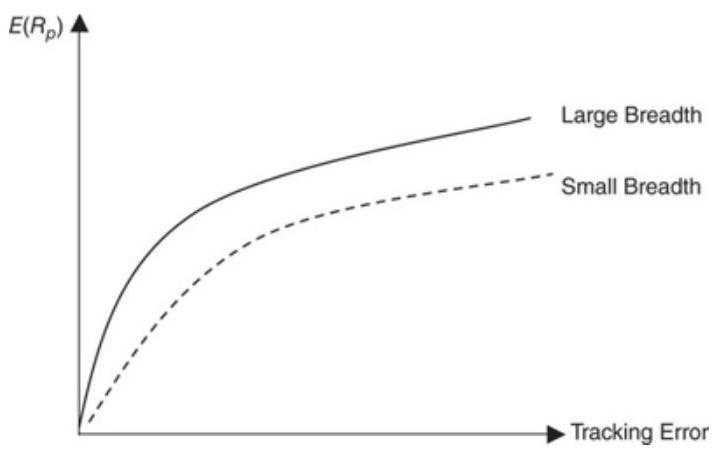
\includegraphics[max width=\textwidth]{2024_04_09_a4726897464687359564g-3}
\end{center}

Expected Return, Tracking Error, and Breadth

\section*{The Limits to Arbitrage}
If the anomalies are as well-known as indicated in this session, and if the trading of anomalies moves security pricing toward more efficient pricing, then why aren't these profits arbitraged away? The answer lies in the limits to arbitrage, which is nicely summarized by Singal. ${ }^{2}$ See Singal, Beyond the Random Walk. The limits to arbitrage refer to the potential inability or unwillingness of speculators, such as equity hedge fund managers, to hold their positions without time constraints or to increase their positions without size constraints. Taking higher portfolio risks through higher leverage increases expected return but there is a limit to the risk that an arbitrager can tolerate and/or is allowed to take. This provides a limit on the level of arbitrage activity by a single manager.

As discussed in this session, many equity hedge fund managers attempt to arbitrage mispriced equities by taking simultaneous and aggressive long and short positions. These portfolios underperform when the subsequent return spreads between the long positions and the short positions are the reverse of the forecasted tendencies. However, even though the basis for a strategy may include well-established historical tendencies, or the hedge fund manager may have discovered truly overvalued or undervalued stocks, the periods of loss can be long and severe. For example, one of the longest observed anomalies was the tendency of value stocks to outperform growth stocks in the United States for many decades prior to 1998. But from January 1998 to early 2000, large U.S. growth stocks outperformed large U.S. value stocks by well over $50 \%$. Value stocks as a group lost money over periods of time in which the most aggressive large-cap growth stocks were experiencing triple-digit gains.

Managers with aggressive bets that value stocks would outperform growth stocks ran the risk of ruin. In other words, a manager who placed a substantial bet that value stocks would revert to their long-term tendency to outperform growth stocks either abandoned the bet or was ruined. Managers who want to be successful in the long run must limit the risk of a fund; by doing so, they provide one of the reasons for the limit to arbitrage. The success of growth stocks in the late 1990s was short-lived. Within approximately one year (by early 2001), the superior performance of growth stocks from 1998 to early 2000 had been fully eroded. And in the 10 years following 2001, value stocks continued their tendency toward higher returns.

Finally, market structures may prevent successful arbitrage in some cases. Especially in micro-cap stocks, institutional investors may be too large to participate, as a $\$ 1$ billion fund may find that the impact of its trading on a stock with a $\$ 50$ million market capitalization may be too large. For stocks with small market capitalization, the liquidity is typically low. Low liquidity means that the bid-ask spread is wide, the volume is thin, and the market impact of a large order can be prohibitive. Market impact is the degree of the short-term effect of trades on the sizes and levels of bid prices and offer prices. Studies of market anomalies must be careful to properly account for the total transaction costs, including the effect of market impact, before concluding that an anomaly is truly profitable.

Another limit to arbitrage is restrictions on short selling in some stocks or even in entire markets. Some countries do not allow short selling. Even in developed markets, short-term bans on short sales may be enacted. Stocks floating recent IPOs or spin-offs may not have shares available to be shorted. Finally, the shares of some companies may be temporarily unavailable for borrowing when the demand to sell the shares short exceeds the supply of borrowable shares. Whenever it is not feasible to sell short shares of a specific firm, the firm may be obviously overvalued but can remain at that valuation for a very long time, as investors do not have a mechanism to profit from the stock's return to a fair value.


\end{document}